%\documentclass{standalone}

%%%%%%%
%	Præambel
%%%%%%

%\documentclass{report}

%	Pakker

\usepackage[utf8]{inputenc}
\usepackage[T1]{fontenc}
\usepackage{graphicx}
\usepackage[cc]{titlepic}
\usepackage{verbatim}
\usepackage{lipsum}
\usepackage{rotating}
\usepackage{fancyvrb}
\usepackage{titling}
\usepackage{listings}
\usepackage{hyperref}
\usepackage[dvipsnames,table]{xcolor}
\usepackage{pdfpages}
\usepackage{float}
\usepackage[danish]{babel}
\usepackage{datetime}
\usepackage{tabularx}
\usepackage{newclude}
\usepackage{tikz}
\usepackage{tablefootnote}

%	Bibloteker

\usetikzlibrary{shapes, arrows}

%	Opsætning

\graphicspath{{./billeder/}}

%	kommandoer

\newcommand{\pic}[2][png]{
	\includegraphics[width=\textwidth]{./#2.#1}
}

\newcommand{\fragCom}[1]{
	\textcolor{LimeGreen}{\texttt{\textbf{#1}}}
}

\newcommand{\logDay}[2][2]{\section*{\formatdate{#2}{#1}{2023}}}

%environmental setup

\lstset{
	breaklines=true,
	breakatwhitespace=true,
	texcl=true,
	extendedchars=false,
	frame=single,
	tabsize=2
}

\lstset{literate=%
	{æ}{{\ae}}1
	{ø}{{\o}}1
	{å}{{\aa}}1
}

%	titel and Aarhus Tech titlecard
\newcommand{\writer}{Sune Koch Rønnow}
%\newcommand{\advisor}{Rasmus Ladefoged Wolffram \& Kenneth Løvgren}
\newcommand{\advisorTwo}{Rasmus Ladefoged Wolffram}
\newcommand{\advisorOne}{Kenneth Løvgren}
\newcommand{\advisor}{\advisorOne{} \& \advisorTwo{}}
\newcommand{\projectName}{ObliGentle}
\newcommand{\reportType}{unavngivenreport}
\newcommand{\reportName}{
	\projectName{}: \reportType{}
}

\newcommand{\subtitle}[1]{%
	\posttitle{%
		\par\end{center}
	\begin{center}\large#1\end{center}
	\vskip0.5em}%
}

\title{\reportName{}}
\subtitle{Svendeprøve ved \\ \advisorOne{} \\ \& \\ \advisorTwo{} \\ \vspace{0.75\baselineskip} Aarhus Tech}
\author{\writer{} \\ sune@kochroennow.dk}
\date{\today}
%\date{\formatdate{6}{10}{2023}}

\newcommand{\makeTechTitlecard}{
	\chapter*{Titelblad}
	\begin{table}[h]
	\center
	\begin{tabularx}{\textwidth}{p{.3\linewidth} X}
	\textbf{Deltagere}		&	\writer{}												\\
	\textbf{Projektnavn} 	&	\projectName{}											\\
	\textbf{Skole}			&	Aarhus Tech \newline{} Hasselager Allé 2, 8260 Viby J	    \\
	\textbf{Projektperiode}	&	\formatdate{13}{11}{2023} - \formatdate{15}{12}{2023}		\\
	\textbf{Afleveringsdato}&	\formatdate{8}{12}{2023}									\\
	\textbf{Vejleder}		&	\advisor{}												\\
	\end{tabularx}
	\end{table}
	\section*{Underskrifter}
	\vspace{3\baselineskip}
	\hrule
	\noindent\small \writer{} \null\hfill Dato\\
	\vspace{2\baselineskip}
	\hrule
	\noindent\small \advisorOne{} \null\hfill Dato\\
	\vspace{2\baselineskip}
	\hrule
	\noindent\small \advisorTwo{} \null\hfill Dato\\
}

% tikz setup

\tikzstyle{terminator} = [rectangle, draw, text centered, rounded corners, minimum height=2em, fill=Magenta!40]
\tikzstyle{process} = [rectangle, draw, text centered, minimum height=2em, fill=Blue!40]
\tikzstyle{positive} = [rectangle, draw, text centered, minimum height=2em, fill=Green!40]
\tikzstyle{negative} = [rectangle, draw, text centered, minimum height=2em, fill=Red!40]
\tikzstyle{decision} = [diamond, draw, text centered, minimum height=2em, fill=Yellow!40]
\tikzstyle{input}=[trapezium, draw, text centered, trapezium left angle=60, trapezium right angle=120, minimum height=2em, fill=Cyan!40]
\tikzstyle{connector} = [draw, -latex']
\tikzstyle{semiConnector} = [draw, -latex',dotted]

%\usepackage{tikz}
%\usetikzlibrary{shapes, arrows}
%\usepackage{verbatim}

\begin{comment}
\tikzstyle{terminator} = [rectangle, draw, text centered, rounded corners, minimum height=2em, fill=Magenta!40]
\tikzstyle{process} = [rectangle, draw, text centered, minimum height=2em, fill=Blue!40]
\tikzstyle{positive} = [rectangle, draw, text centered, minimum height=2em, fill=Green!40]
\tikzstyle{negative} = [rectangle, draw, text centered, minimum height=2em, fill=Red!40]
\tikzstyle{decision} = [diamond, draw, text centered, minimum height=2em, fill=Yellow!40]
\tikzstyle{input}=[trapezium, draw, text centered, trapezium left angle=60, trapezium right angle=120, minimum height=2em, fill=Cyan!40]
\tikzstyle{connector} = [draw, -latex']
\tikzstyle{semiConnector} = [draw, -latex',dotted]
\end{comment}

\begin{center}
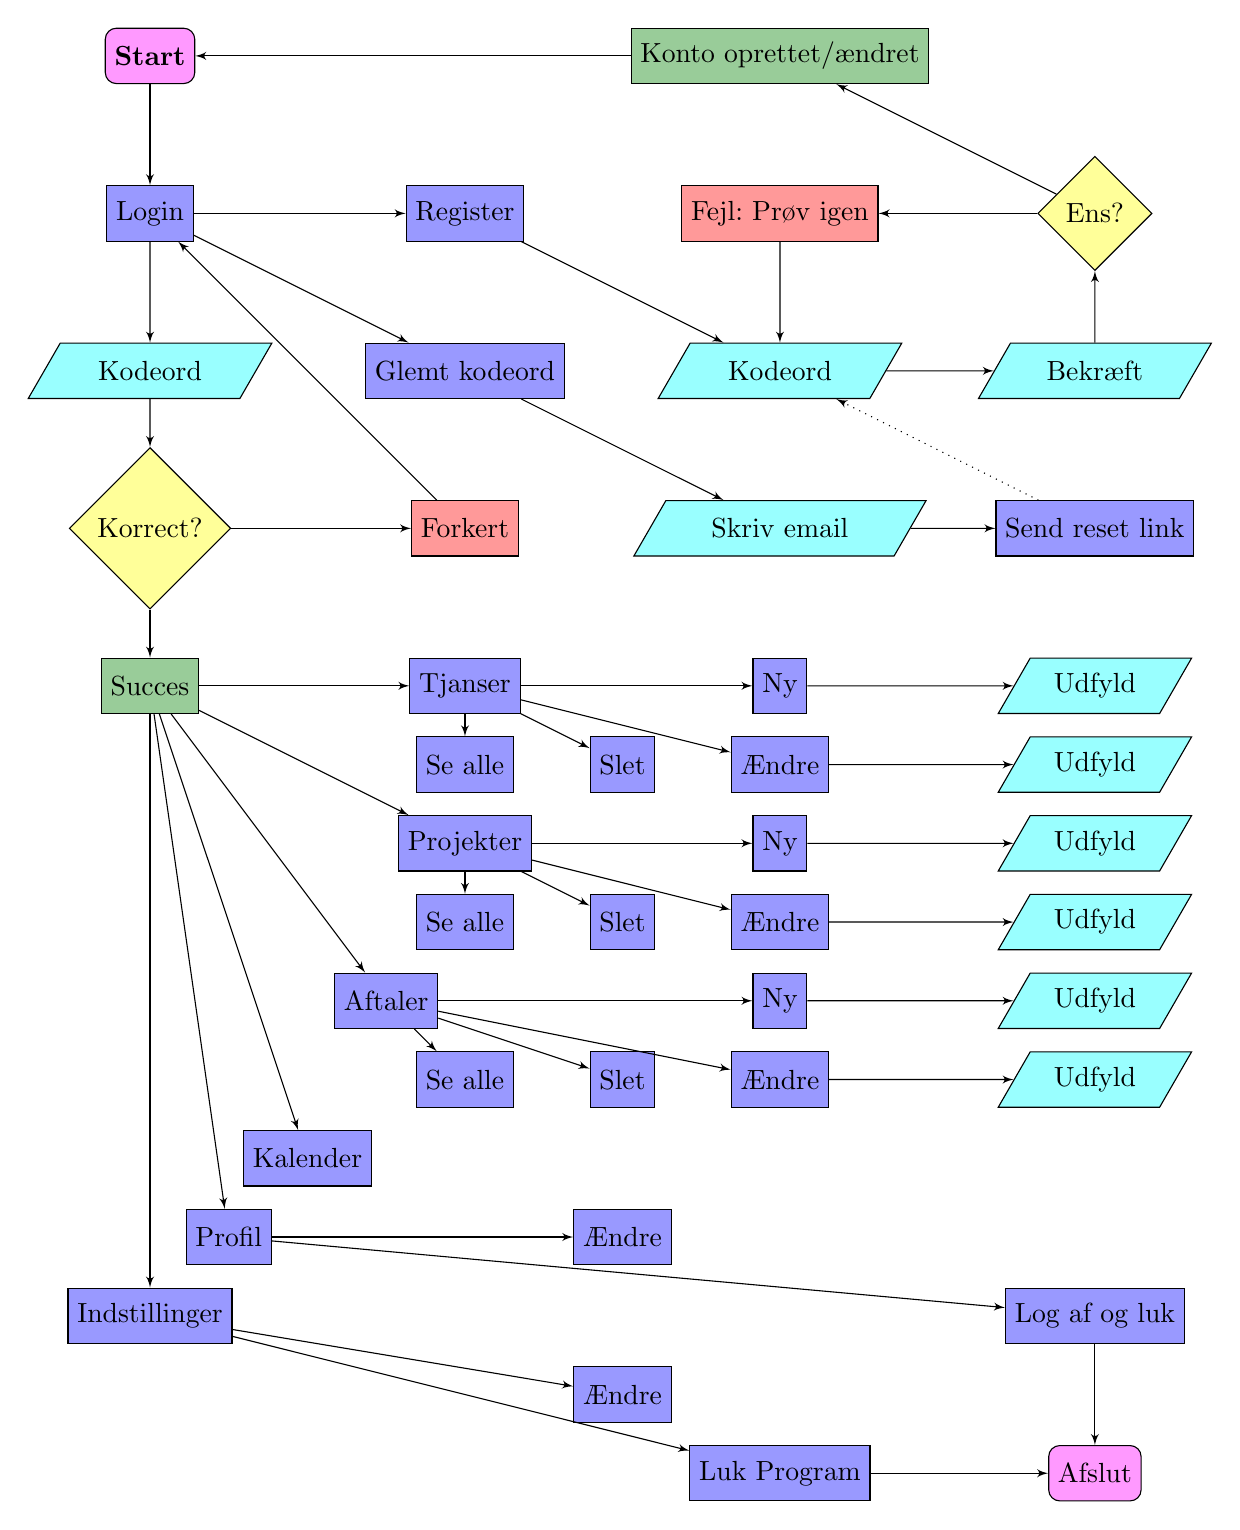
\begin{tikzpicture}

\node[terminator] at (0,0) (start) {\textbf{Start}};

\node[process] at (0,-2) (haveLogin) {Login};

\node[process] at (4,-2) (signUp) {Register};
\node[input] at (8,-4) (inputPass) {Kodeord};
\node[input] at (12,-4) (confirmPass) {Bekræft};
\node[decision] at (12,-2) (matchPass) {Ens?};
\node[positive] at (8,0) (createAcc) {Konto oprettet/ændret};
\node[negative] at (8,-2) (passAgain) {Fejl: Prøv igen};


\node[input] at (0,-4) (havePass) {Kodeord};
\node[process] at (4,-4) (forgottenPass) {Glemt kodeord};
\node[input] at (8,-6) (resetPassEmail) {Skriv email};
\node[process] at (12,-6) (resetPassSent) {Send reset link};

\node[decision] at (0,-6) (passCorrect) {Korrect?};
\node[negative] at (4,-6) (passCorrectNo) {Forkert};
\node[positive] at (0,-8) (passCorrectYes) {Succes};

\node[process] at (4,-8) (chores) {Tjanser};
\node[process] at (8,-8) (choresCreate) {Ny};
\node[input] at (12,-8) (choresCreateInput) {Udfyld};
\node[process] at (8,-9) (choresChange) {Ændre};
\node[input] at (12,-9) (choresChangeInput) {Udfyld};
\node[process] at (4,-9) (choresView) {Se alle};
\node[process] at (6,-9) (choresDelete) {Slet};

\path [connector] (chores) -- (choresCreate);
\path [connector] (choresCreate) -- (choresCreateInput);
\path [connector] (chores) -- (choresChange);
\path [connector] (choresChange) -- (choresChangeInput);
\path [connector] (chores) -- (choresView);
\path [connector] (chores) -- (choresDelete);


\node[process] at (4,-10) (projects) {Projekter};
\node[process] at (8,-10) (projectsCreate) {Ny};
\node[input] at (12,-10) (projectsCreateInput) {Udfyld};
\node[process] at (8,-11) (projectsChange) {Ændre};
\node[input] at (12,-11) (projectsChangeInput) {Udfyld};
\node[process] at (4,-11) (projectsView) {Se alle};
\node[process] at (6,-11) (projectsDelete) {Slet};

\path [connector] (projects) -- (projectsCreate);
\path [connector] (projectsCreate) -- (projectsCreateInput);
\path [connector] (projects) -- (projectsChange);
\path [connector] (projectsChange) -- (projectsChangeInput);
\path [connector] (projects) -- (projectsView);
\path [connector] (projects) -- (projectsDelete);


\node[process] at (3,-12) (appointments) {Aftaler};
\node[process] at (8,-12) (appointmentsCreate) {Ny};
\node[input] at (12,-12) (appointmentsCreateInput) {Udfyld};
\node[process] at (8,-13) (appointmentsChange) {Ændre};
\node[input] at (12,-13) (appointmentsChangeInput) {Udfyld};
\node[process] at (4,-13) (appointmentsView) {Se alle};
\node[process] at (6,-13) (appointmentsDelete) {Slet};

\path [connector] (appointments) -- (appointmentsCreate);
\path [connector] (appointmentsCreate) -- (appointmentsCreateInput);
\path [connector] (appointments) -- (appointmentsChange);
\path [connector] (appointmentsChange) -- (appointmentsChangeInput);
\path [connector] (appointments) -- (appointmentsView);
\path [connector] (appointments) -- (appointmentsDelete);



\node[process] at (2,-14) (calendar) {Kalender};

\node[process] at (1,-15) (profile) {Profil};
\node[process] at (6,-15) (profileChange) {Ændre};
\node[process] at (12,-16) (profileLogout) {Log af og luk};

\node[process] at (0,-16) (settings) {Indstillinger};
\node[process] at (6, -17) (settingsChange) {Ændre};
\node[process] at (8,-18) (settingsTerm) {Luk Program};

\node[terminator] at (12,-18) (end) {Afslut};

\path [connector] (start) -- (haveLogin);

\path [connector] (haveLogin) -- (signUp);
\path [connector] (signUp) -- (inputPass);
\path [connector] (inputPass) -- (confirmPass);
\path [connector] (confirmPass) -- (matchPass);
\path [connector] (matchPass) -- (createAcc);
\path [connector] (matchPass) -- (passAgain);
\path [connector] (passAgain) -- (inputPass);
\path [connector] (createAcc) -- (start);

\path [connector] (haveLogin) -- (havePass);
\path [connector] (haveLogin) -- (forgottenPass);
\path [connector] (forgottenPass) -- (resetPassEmail);
\path [connector] (resetPassEmail) -- (resetPassSent);
\path [semiConnector] (resetPassSent) -- (inputPass);


\path [connector] (havePass) -- (passCorrect);
\path [connector] (passCorrect) -- (passCorrectNo);
\path [connector] (passCorrectNo) -- (haveLogin);
\path [connector] (passCorrect) -- (passCorrectYes);

\path [connector] (passCorrectYes) -- (chores);
\path [connector] (passCorrectYes) -- (projects);
\path [connector] (passCorrectYes) -- (appointments);
\path [connector] (passCorrectYes) -- (calendar);

\path [connector] (passCorrectYes) -- (profile);
\path [connector] (profile) -- (profileLogout);
\path [connector] (profile) -- (profileChange);
\path [connector] (profileLogout) -- (end);

\path [connector] (passCorrectYes) -- (settings);
\path [connector] (settings) -- (settingsTerm);
\path [connector] (settings) -- (settingsChange);
\path [connector] (settingsTerm) -- (end);




\end{tikzpicture}

\begin{comment}
\node [data] at (0,-2) (data) {Provide data};
\node [decision] at (0,-5) (decision) {Valid data?};
\node [error] at (3.5,-5) (error) {Error};
\node [success] at (0,-8) (success) {Success};
\node [terminator] at (0,-10) (end) {\textbf{End}};
\node[draw=none] at (1.85, -4.75) (no) {No};
\node[draw=none] at (0.35, -6.75) (yes) {Yes};



\path [connector] (start) -- (data);
\path [connector] (data) -- (decision);
\path [connector] (decision) -- (error);
\path [connector] (decision) -- (success);
\path [connector] (error) |- (end);
\path [connector] (success) -- (end);
\end{comment}


\end{center}